% SafeMAP v2 pipeline (Fig. 1). Build: pdflatex Fig1.tex
% Drawn at final size (include at scale 1): smallest text is 8 pt, as the
% journal requires.
\documentclass[tikz,border=2pt]{standalone}
\usepackage[scaled]{helvet}
\renewcommand{\familydefault}{\sfdefault}
\usepackage[none]{hyphenat}
\usetikzlibrary{positioning,arrows.meta,calc}
\definecolor{ink}{HTML}{1F3A56}
\definecolor{step}{HTML}{EAF1F7}
\definecolor{dec}{HTML}{FFF4DE}
\definecolor{decb}{HTML}{8A6212}
\definecolor{llm}{HTML}{EFE9F7}
\definecolor{llmb}{HTML}{5A3E82}
\definecolor{rej}{HTML}{A33A27}
\definecolor{rejf}{HTML}{FBECE8}
\definecolor{acc}{HTML}{23663F}
\definecolor{accf}{HTML}{E6F4EA}
\definecolor{lane}{HTML}{F3F1F8}
\begin{document}
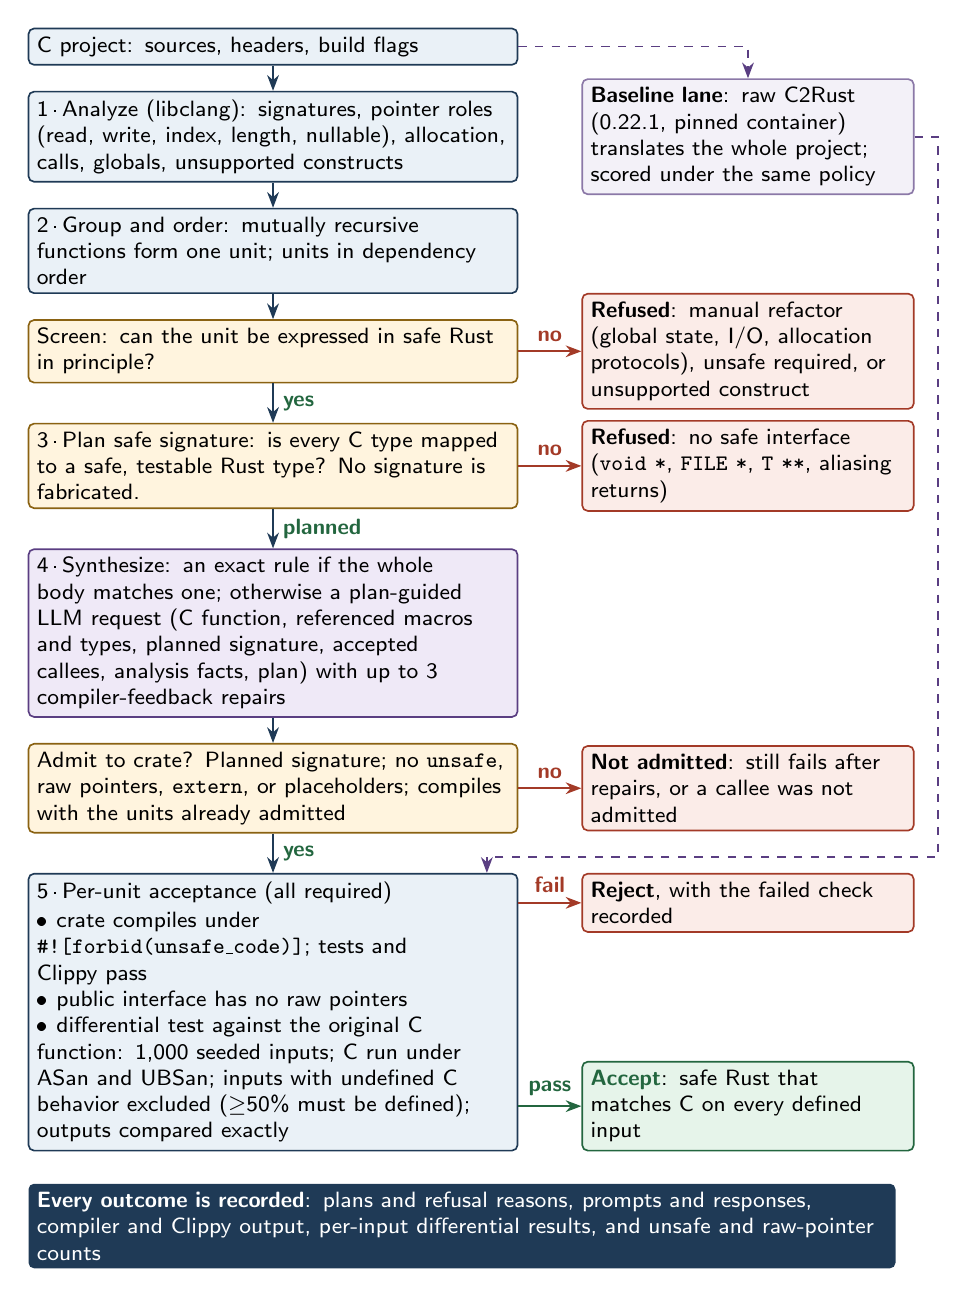
\begin{tikzpicture}[
  font=\footnotesize, node distance=3.2mm,
  >={Stealth[length=2mm]}, line width=0.6pt,
  base/.style={rounded corners=2pt, align=left, inner sep=3pt, text width=#1},
  box/.style={base=60mm, draw=ink, fill=step},
  dec/.style={base=60mm, draw=decb, fill=dec},
  gen/.style={base=60mm, draw=llmb, fill=llm},
  rejbox/.style={base=40mm, draw=rej, fill=rejf},
  hd/.style={font=\small\bfseries},
  flow/.style={->, draw=ink},
  no/.style={->, draw=rej},
  lbl/.style={font=\footnotesize\bfseries, text=#1},
]
% ---- Main flow (left column) ----------------------------------------------
\node[box] (in) {{\hd C project}: sources, headers, build flags};
\node[box, below=of in] (an) {{\hd 1\,\textperiodcentered\,Analyze} (libclang): signatures,
  pointer roles (read, write, index, length, nullable), allocation, calls,
  globals, unsupported constructs};
\node[box, below=of an] (gr) {{\hd 2\,\textperiodcentered\,Group and order}: mutually
  recursive functions form one unit; units in dependency order};
\node[dec, below=of gr] (sc) {{\hd Screen}: can the unit be expressed in safe
  Rust in principle?};
\node[dec, below=5mm of sc] (pl) {{\hd 3\,\textperiodcentered\,Plan safe signature}: is every
  C type mapped to a safe, testable Rust type? No signature is fabricated.};
\node[gen, below=5mm of pl] (sy) {{\hd 4\,\textperiodcentered\,Synthesize}: an exact rule if
  the whole body matches one; otherwise a plan-guided LLM request (C function,
  referenced macros and types, planned signature, accepted callees, analysis
  facts, plan) with up to 3 compiler-feedback repairs};
\node[dec, below=of sy] (ad) {{\hd Admit to crate?} Planned signature; no
  \texttt{unsafe}, raw pointers, \texttt{extern}, or placeholders; compiles
  with the units already admitted};
\node[box, below=5mm of ad] (va) {{\hd 5\,\textperiodcentered\,Per-unit acceptance} (all required)\\[1pt]
  \textbullet\ crate compiles under \texttt{\#![forbid(unsafe\_code)]}; tests
  and Clippy pass\\
  \textbullet\ public interface has no raw pointers\\
  \textbullet\ differential test against the original C function: 1,000
  seeded inputs; C run under ASan and UBSan; inputs with undefined C behavior
  excluded ($\geq$50\% must be defined); outputs compared exactly};

\draw[flow] (in) -- (an);
\draw[flow] (an) -- (gr);
\draw[flow] (gr) -- (sc);
\draw[flow] (sc) -- node[lbl=acc, right]{yes} (pl);
\draw[flow] (pl) -- node[lbl=acc, right]{planned} (sy);
\draw[flow] (sy) -- (ad);
\draw[flow] (ad) -- node[lbl=acc, right]{yes} (va);

% ---- Outcomes (right column) ------------------------------------------------
\node[rejbox, right=8mm of sc] (r1) {{\bfseries Refused}: manual refactor
  (global state, I/O, allocation protocols), unsafe required, or unsupported
  construct};
\node[rejbox, right=8mm of pl] (r2) {{\bfseries Refused}: no safe interface
  (\texttt{void *}, \texttt{FILE *}, \texttt{T **}, aliasing returns)};
\node[rejbox, right=8mm of ad] (r3) {{\bfseries Not admitted}: still fails after
  repairs, or a callee was not admitted};
\node[rejbox, right=8mm of va.north east, anchor=north west] (bad) {{\bfseries Reject}, with the
  failed check recorded};
\node[base=40mm, draw=acc, fill=accf, right=8mm of va.south east, anchor=south west]
  (ok) {{\bfseries\color{acc} Accept}: safe Rust that matches C on every defined input};

\draw[no] (sc) -- node[lbl=rej, above]{no} (r1);
\draw[no] (pl) -- node[lbl=rej, above]{no} (r2);
\draw[no] (ad) -- node[lbl=rej, above]{no} (r3);
\draw[no] (va.east |- bad.west) -- node[lbl=rej, above]{fail} (bad.west);
\draw[->, draw=acc] (va.east |- ok.west) -- node[lbl=acc, above]{pass} (ok.west);

% ---- C2Rust reference lane -------------------------------------------------
\node[base=40mm, draw=llmb!70, fill=lane, right=8mm of an] (c2) {{\bfseries Baseline
  lane}: raw C2Rust (0.22.1, pinned container) translates the whole project;
  scored under the same policy};
\draw[->, dashed, draw=llmb] (in.east) -| (c2.north);
\coordinate (rail) at ($(c2.east)+(3mm,0)$);
\draw[->, dashed, draw=llmb] (c2.east) -- (rail) |- ($(bad.north)+(0,2mm)$)
  -| ($(va.north east)+(-4mm,0)$);

% ---- Recording -------------------------------------------------------------
\node[fill=ink, text=white, rounded corners=2pt, inner sep=3pt, align=left,
  text width=108mm, anchor=north west] at ($(va.south west)+(0,-4mm)$) (rec)
  {{\bfseries Every outcome is recorded}: plans and refusal reasons, prompts and
  responses, compiler and Clippy output, per-input differential results, and
  unsafe and raw-pointer counts};
\end{tikzpicture}
\end{document}
